%% fig_roadmap.tex   (generated by make_round41.py; do not edit by hand)
%% The five parts of the paper and the two theorems they lead to.
\documentclass[tikz,border=8pt]{standalone}
\usepackage{amsmath,amssymb}
\usetikzlibrary{arrows.meta,calc,decorations.pathreplacing}
%% palette.tex -- shared colour definitions for the figures
\definecolor{PInk}{RGB}{26,32,44}
\definecolor{PBlue}{RGB}{37,82,139}
\definecolor{PTeal}{RGB}{23,127,125}
\definecolor{POchre}{RGB}{193,138,44}
\definecolor{PClay}{RGB}{178,74,58}
\definecolor{PSlate}{RGB}{108,122,137}
\definecolor{PViolet}{RGB}{110,86,150}
\definecolor{WBlue}{RGB}{223,234,246}
\definecolor{WTeal}{RGB}{220,238,236}
\definecolor{WOchre}{RGB}{250,240,218}
\definecolor{WClay}{RGB}{247,229,224}
\definecolor{WSlate}{RGB}{238,241,244}
\definecolor{PMag}{RGB}{158,58,110}
\definecolor{PGrass}{RGB}{62,124,66}
\definecolor{PAmber}{RGB}{214,112,38}
\definecolor{PIndigo}{RGB}{58,64,140}
\definecolor{PRule}{RGB}{176,186,197}

%% shared macros so the standalone figures match the paper
\providecommand{\QQ}{\mathbb{Q}}
\providecommand{\ZZ}{\mathbb{Z}}
\providecommand{\RR}{\mathbb{R}}
\providecommand{\CC}{\mathbb{C}}
\providecommand{\PP}{\mathbb{P}}
\providecommand{\Kx}{K^{\times}}
\providecommand{\HW}{W}
\providecommand{\Nm}{\mathrm{N}}
\providecommand{\Hdg}{\mathrm{Hdg}}
\providecommand{\NS}{\mathrm{NS}}
\providecommand{\cA}{\mathcal{A}}
\providecommand{\cD}{\mathcal{D}}
\providecommand{\cF}{\mathcal{F}}
\providecommand{\cP}{\mathcal{P}}
\providecommand{\cO}{\mathcal{O}}
\providecommand{\cQ}{\mathcal{Q}}
\providecommand{\bbar}[1]{\overline{#1}}
\providecommand{\ch}{\operatorname{ch}}
\providecommand{\End}{\mathrm{End}}
\providecommand{\Ext}{\operatorname{Ext}}
\providecommand{\Supp}{\operatorname{Supp}}

\begin{document}
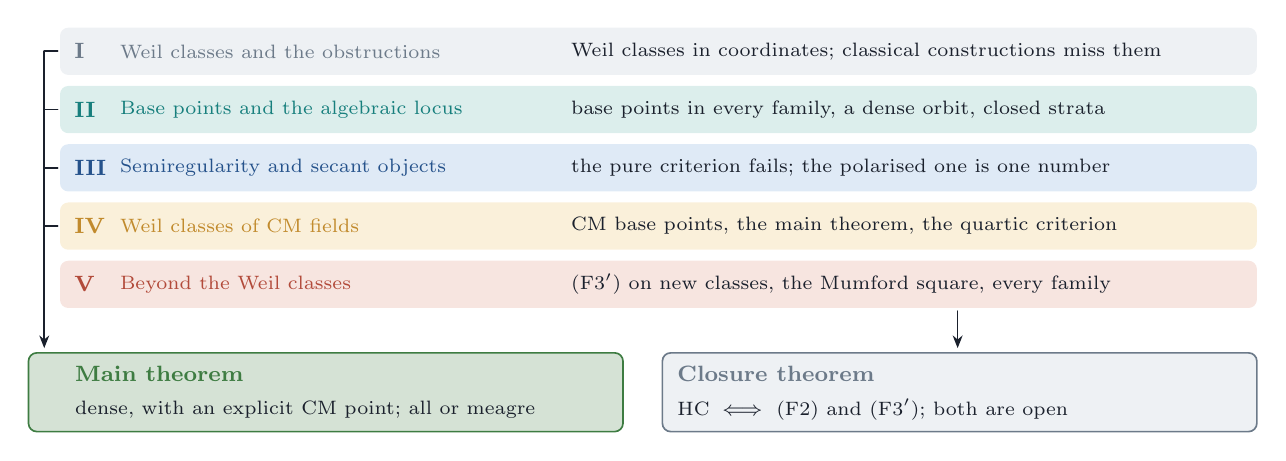
\begin{tikzpicture}[x=1cm,y=1cm,line join=round,line cap=round,
  font=\small,text=PInk,lbl/.style={inner sep=1pt}]
  \path[fill=WSlate,draw=none,rounded corners=3.0pt] (0.4000,4.5800) rectangle (15.6000,5.1800);
  \path[fill=WTeal,draw=none,rounded corners=3.0pt] (0.4000,3.8400) rectangle (15.6000,4.4400);
  \path[fill=WBlue,draw=none,rounded corners=3.0pt] (0.4000,3.1000) rectangle (15.6000,3.7000);
  \path[fill=WOchre,draw=none,rounded corners=3.0pt] (0.4000,2.3600) rectangle (15.6000,2.9600);
  \path[fill=WClay,draw=none,rounded corners=3.0pt] (0.4000,1.6200) rectangle (15.6000,2.2200);
  \path[fill=PGrass!22!white,draw=PGrass,line width=0.60pt,rounded corners=3.0pt] (0.0000,0.0500) rectangle (7.5500,1.0500);
  \path[fill=WSlate,draw=PSlate,line width=0.60pt,rounded corners=3.0pt] (8.0500,0.0500) rectangle (15.6000,1.0500);
  \draw[PInk,line width=0.6pt,-{Stealth[length=4.6pt,width=3.6pt]}] (0.2000,4.8800) -- (0.2000,1.1100);
  \draw[PInk,line width=0.6pt] (0.2000,4.8800) -- (0.3700,4.8800);
  \draw[PInk,line width=0.6pt] (0.2000,4.1400) -- (0.3700,4.1400);
  \draw[PInk,line width=0.6pt] (0.2000,3.4000) -- (0.3700,3.4000);
  \draw[PInk,line width=0.6pt] (0.2000,2.6600) -- (0.3700,2.6600);
  \draw[PInk,line width=0.6pt,-{Stealth[length=4.6pt,width=3.6pt]}] (11.8000,1.5800) -- (11.8000,1.1100);
  \node[lbl,anchor=west,text=PSlate,font=\footnotesize] at (0.5400,4.8800) {\textbf{I}};
  \node[lbl,anchor=west,text=PSlate,font=\scriptsize] at (1.1200,4.8800) {Weil classes and the obstructions};
  \node[lbl,anchor=west,text=PInk,font=\scriptsize] at (6.8500,4.8800) {Weil classes in coordinates; classical constructions miss them};
  \node[lbl,anchor=west,text=PTeal,font=\footnotesize] at (0.5400,4.1400) {\textbf{II}};
  \node[lbl,anchor=west,text=PTeal,font=\scriptsize] at (1.1200,4.1400) {Base points and the algebraic locus};
  \node[lbl,anchor=west,text=PInk,font=\scriptsize] at (6.8500,4.1400) {base points in every family, a dense orbit, closed strata};
  \node[lbl,anchor=west,text=PBlue,font=\footnotesize] at (0.5400,3.4000) {\textbf{III}};
  \node[lbl,anchor=west,text=PBlue,font=\scriptsize] at (1.1200,3.4000) {Semiregularity and secant objects};
  \node[lbl,anchor=west,text=PInk,font=\scriptsize] at (6.8500,3.4000) {the pure criterion fails; the polarised one is one number};
  \node[lbl,anchor=west,text=POchre,font=\footnotesize] at (0.5400,2.6600) {\textbf{IV}};
  \node[lbl,anchor=west,text=POchre,font=\scriptsize] at (1.1200,2.6600) {Weil classes of CM fields};
  \node[lbl,anchor=west,text=PInk,font=\scriptsize] at (6.8500,2.6600) {CM base points, the main theorem, the quartic criterion};
  \node[lbl,anchor=west,text=PClay,font=\footnotesize] at (0.5400,1.9200) {\textbf{V}};
  \node[lbl,anchor=west,text=PClay,font=\scriptsize] at (1.1200,1.9200) {Beyond the Weil classes};
  \node[lbl,anchor=west,text=PInk,font=\scriptsize] at (6.8500,1.9200) {(F3$'$) on new classes, the Mumford square, every family};
  \node[lbl,anchor=west,text=PGrass,font=\footnotesize] at (0.5500,0.7800) {\textbf{Main theorem}};
  \node[lbl,anchor=west,text=PInk,font=\scriptsize] at (0.5500,0.3300) {dense, with an explicit CM point; all or meagre};
  \node[lbl,anchor=west,text=PSlate,font=\footnotesize] at (8.2000,0.7800) {\textbf{Closure theorem}};
  \node[lbl,anchor=west,text=PInk,font=\scriptsize] at (8.2000,0.3300) {$\mathrm{HC}\iff$ (F2) and (F3$'$); both are open};
\end{tikzpicture}
\end{document}
